\section{A local spanner for axis parallel squares}
\seclab{squares}

One can modify the above construction for axis-parallel squares, and
get a local spanner without dependency on the spread.

\subsubsection{Construction}

The input is a point set $\PS$ of $n$ points in the plane, and an
approximation parameter $\eps \in (0,1/2)$.  We assume that the input
point set $\PS$ is in general position. Specifically, no two points of
$\PS$ share a coordinate value, or appear in opposing corners of an
axis-parallel square -- this can be ensured by slightly perturbing the
points if necessary (or symbolic perturbation). Let
$\Binfty = [-1,1]^2$ be the unit ``ball'' under the $L_\infty$
norm.

Let $\epsA = \eps/20$.  The algorithm computes a $1/\epsA$-\SSPD
$\WS$, using the algorithm of \thmref{S:S:P:D:main}. By using the
algorithm of \lemref{refine:d:w}, and increasing the weight and number
of pairs by a factor of $\Of(1/\epsA)$, one can assume that every pair
$\{ \PSX, \PSY \} \in \WS$ is not only semi-separated, but also that
there is an associated double wedge of angle $\leq \epsA$ containing
$\PSX$ and $\PSY$ in opposing wedges, using the algorithm of
\lemref{refine:d:w}.  The algorithm now computes $\Binfty$-Delaunay
triangulation, see \defref{c:del:triang}, for each such pair, and adds
the edges of the triangulation to the resulting graph $\G$.



\subsubsection{Analysis}

\paragraph{Size and running time}

Computing the \SSPD takes $\Of\pth{n \epsA^{-2} \log n}$ time, and the
refinement takes $\Of\pth{n \epsA^{-3} \log n}$ time (which is also
the weight of the resulting \SSPD). The number of edges of each
$L_\infty$-Delaunay triangulation for a pair is proportional to its
weight, which implies that the total number of edges in the resulting
graph $\G$ is $\Of\pth{ \epsA^{-3} n\log n}$. Computing all these
Delaunay triangulations takes $\Of\pth{ \epsA^{-3}n \log^2 n}$ time.


\paragraph{Shrinking squares}
We need the following lemma about the shrinking of axis-parallel
squares.  Observe that this property definitely does not hold for
disks, as illustrated in \figref{bad}.

\begin{lemma}
    \lemlab{shrink:squars}%
    %
    (A) Let $\sqr$ be an axis parallel square in the plane, and let
    $\pa, \pb$ be two arbitrary points in $\sqr$. Then, there is a
    square $\sqrA \subseteq \sqr$ that contains $\pa$ and $\pb$ on its
    boundary.

    (B) Let $\sqr$ be as before, and let $\PSX, \PSY$ be two point
    sets in the plane, such that
    $\PSX' = \PSX \cap \sqr \neq \emptyset$ and
    $\PSY' = \PSY \cap \sqr \neq \emptyset$. Let
    $\px \in \PSX, \py \in \PSY$ be the two points realizing
    $\dsZ{\infty}{\PSX'}{\PSY'} = \underset{\pa \in \PSX', \pb \in
       \PSY'}{\min} \dZ{\infty}{\pa}{\pb}$. Then, there is a square
    $\sqrA \subseteq \sqr$ that contains $\px$ and $\py$ on its
    boundary, and $\sqrA$ does not contain any other point of
    $\PSX \cup \PSY$.
\end{lemma}
\begin{proof}
    (A) Start shrinking $\sqr$ around its center till it contains one
    of the points (say $\pa$ is on its boundary. Next, move the center
    of the square towards $\pa$ till the boundary of the continuously
    shrinking square passes through $\pb$. If $\pa$ and $\pb$ lie on
    adjacent edges, then continue the shrinking process by moving the
    center towards the common corner of the shared edges -- this
    process stops when one of the points is on the corner of the
    square.  Clearly, the resulting square $\sqrA$ is the desired
    square, see \figref{shrink:sq}.

    \begin{figure}[h]
        \phantom{}\hfill%
        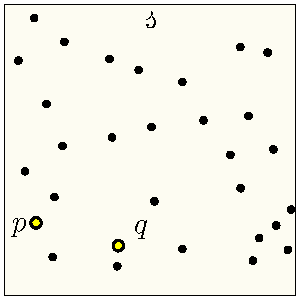
\includegraphics[page=1,width=0.2\linewidth]{figs/shrink_sq}
        \hfill%
        \includegraphics[page=2,width=0.2\linewidth]{figs/shrink_sq}%
        \hfill%
        \includegraphics[page=3,width=0.2\linewidth]{figs/shrink_sq}%
        \hfill%
        \includegraphics[page=4,width=0.2\linewidth]{figs/shrink_sq}
        \hfill\phantom{}%

        \caption{}
        \figlab{shrink:sq}
    \end{figure}

    (B) Let $r = \dsZ{\infty}{\PSX'}{\PSY'}$. By (A), there is a
    square $\sqrA \subseteq \sqr$ having $\px$ and $\py$ on apposing
    sides. As such, the side length of $\sqrA$ is $r$. Assume for
    contradiction, that there is some other point
    $\px' \in \PSX \cap \sqrA$. By our general position assumption,
    $\px'$ is in the interior of $\sqrA$, and in particular,
    $\dZ{\infty}{\px'}{\py} < r$, which is a contradiction to the
    choice of $\px$ and $\py$.
\end{proof}

\paragraph{Local spanner property}
\begin{lemma}
    \lemlab{squares}%
    %
    For any axis parallel square $\sqr$ in the plane, and any two
    points $\pa, \pb \in \PS \cap \sqr$, we have a $(1+\eps)$-path in
    $\restrictY{\G}{\sqr}$.
\end{lemma}
\begin{proof}
    We prove the existence of a $(1+\eps)$-path between every pair
    $x,y\in \PS \cap \sqr$ of points, by induction over the rank of
    $\dY{\px}{\py}$. The base case is simple, as the pair
    $(\{\px\},\{\py\})$ is a pair in $\WS$, and $xy$ is thus an edge
    in $G$. Now, consider two points $\px, \py \in \PS \cap \sqr$,
    where $\sqr$ is some arbitrary square. There exists a pair
    $\Pair = \{ \PSX, \PSY \} \in \WS$ such that $\px \in \PSX$ and
    $\py \in \PSY$, and this pair is $\epsA^{-1}$-semi separated and
    is also separated by a double wedge of angle $\leq \epsA$.  See
    \figref{infty:spanner}.  Furthermore, assume that
    $\diameterX{\PSX} < \diameterX{\PSY}$.

    \begin{figure}[h]
        \hfill%
        {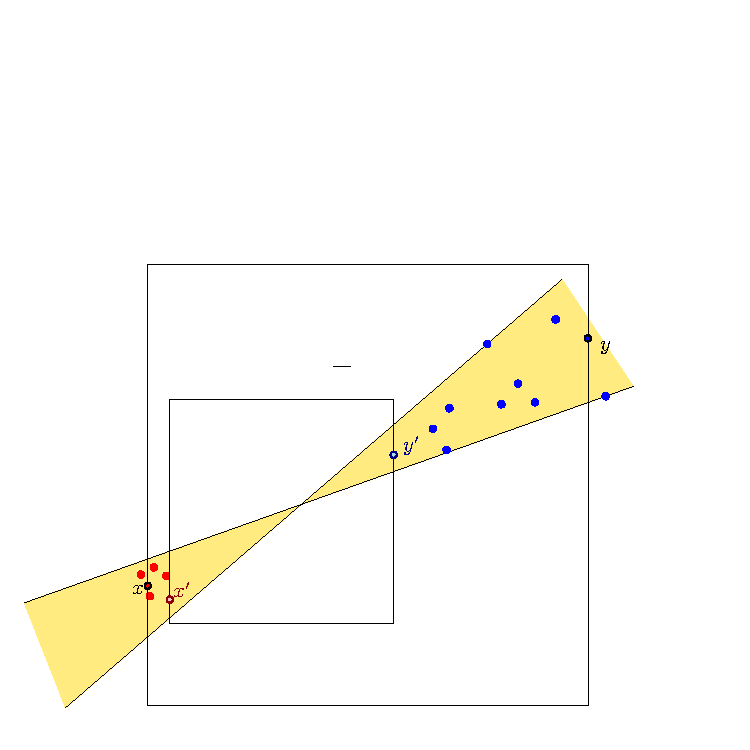
\includegraphics{figs/spanner_sq}} \hfill%
        \phantom{}%
        % 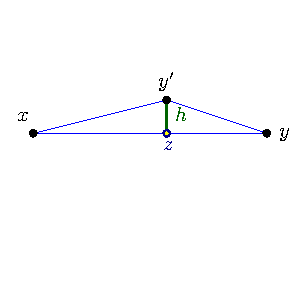
\includegraphics{figs/triangle}%
        \caption{A square region $\sqrA$ and two double-wedge
           semi-separated point sets $\PSX$ (red) and $\PSY$
           (blue. Notice that while $\px'$ and $\py'$ are the closest
           pair using $L_\infty$, that is not necessarily true for the
           Euclidean distance.}
        \figlab{infty:spanner}
    \end{figure}

    Let $\PSX' = \PSX \cap \sqr$ and $\PSY' = \PSY \cap \sqr$, and
    consider the two points $\px' \in \PSX'$ and $\py' \in \PSY'$
    realizing $r = \dsZ{\infty}{\PSX'}{\PSY'}$. By
    \lemref{shrink:squars} there exists a square $\sqrA$ containing
    $\px', \py'$ on its boundary (on two apposing edges), such that
    $\sqrA \subseteq \sqr$, and $\sqrA$ contains no other points
    $\PSX \cup \PSY$. By construction, we have that $\px'\py'$ is in
    the $\Binfty$-Delaunay triangulation of $\Pair$, and thus
    $\px' \py' \in \G$. Since $\dY{\px}{\px'} \ll \dY{\px}{\py}$ we
    have that by induction
    $\dGZ{\G}{\px}{\px'} \leq (1+\eps)\dY{\px}{\px'}$.

    % \newpage


    Let $\ell = \dY{\px'}{\py'}$. Due to the semi-separation property
    and since $\diameterX{\PSX} < \diameterX{\PSY}$,

    \begin{equation*}
        \dY{\px}{\px'}%
        \leq%
        \diameterX{\PSX}%
        \leq%
        \epsA \dY{\PSX}{\PSY}%
        \leq%
        \epsA \sqrt{2} \cdot \dGZ{\infty}{\PSX}{\PSY}%
        \leq
        2
        \epsA \ell.
    \end{equation*}

    Thus, we have that
    \begin{equation*}
        \dGZ{\G}{\px}{\px'}%
        \leq%
        (1+\eps)\dY{\px}{\px'}
        \leq%
        (1+\eps) 2\epsA \ell
        \leq%
        4\epsA \ell.
    \end{equation*}
    By the triangle inequality, we have
    \begin{equation*}
        (1-2\epsA)\ell
        \leq
        \dY{\px'}{\py'} - \dY{\px}{\px'}
        \leq%
        \dY{\px}{\py'}%
        \leq%
        (1+2\epsA)\ell.
    \end{equation*}


    \begin{figure}[h]
        \hfill%
        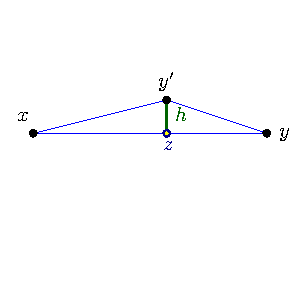
\includegraphics{figs/triangle}%
        \hfill%
        \phantom{}%
        \caption{An illustration of the relative positions of $\px$,
           $\py$, $\py'$, and $\pz$. The angle of the separating
           double-wedge guarantees that $\angle \py' \px \py$ is
           small.}
        \figlab{triangle}
    \end{figure}

    Consider the triangle $\triangle \px \py' \py$, and observe that
    by the double-wedge property
    $\alpha = \angle \py' \px \py \leq \epsA$.  Let $\pz$ be the
    projection of $\py'$ to $\px \py$, and let
    \begin{equation*}
        h%
        =%
        \dY{\py'}{ \pz}%
        =%
        \dY{\px}{\py'} \sin \alpha
        \leq
        \dY{\px}{\py'} \sin \epsA
        \leq%
        \dY{\px}{\py'}  \epsA
        \leq%
        \epsA (1+2 \epsA)\ell
        \leq
        2 \epsA \ell,
    \end{equation*}
    as $\epsA \in (0,1/10)$, the monotonicity of $\sin$ in this range,
    and as $\sin \epsA \leq \epsA$.

    We have that
    $\dY{\px}{\pz} \leq \dY{\px}{\py'} \leq
    (1+2\epsA)\ell$. Similarly, we have
    \begin{equation*}
        \dY{\px}{\pz}%
        =%
        \dY{\px}{\py'} \cos \alpha
        \geq%
        (1-\alpha^2/2)\dY{\px}{\py'}
        \geq
        (1-\epsA^2/2)(1-2\epsA)\ell
        \geq
        (1-3\epsA)\ell.
    \end{equation*}


    By the triangle inequality, we have that
    \begin{equation*}
        \dY{\py'}{\py}
        \geq%
        \dY{\px}{\py}
        -\dY{\py'}{\px}
        \geq%
        \dY{\px}{\py}
        - (1+2\epsA)\ell.
    \end{equation*}
    As for an upper bound, we have
    \begin{align*}
      \dY{\py'}{\py}
      &\leq%
        \dY{\pz}{\py} + h%
        \leq%
        \dY{\px}{\py} - \dY{\px}{\pz} +
        2 \epsA \ell
        \leq
        \dY{\px}{\py} - (1-3\epsA)\ell
        +2 \epsA \ell
      \\&
      =
      \dY{\px}{\py} - (1-5\epsA)\ell
      <%
      \dY{\px}{\py}.
    \end{align*}
    As such, by induction
    $\dGZ{\G}{\py'}{\py} \leq (1+\eps) \dY{\py'}{\py}$.

    We thus have that
    \begin{align*}
      \dGZ{\G}{\px}{\py}%
      &\leq%
        \dGZ{\G}{\px}{\px'} + \dY{\px'}{\py'}
        +
        \dGZ{\G}{\py'}{\py}%
        \leq%
        4\epsA \ell
        +
        \ell
        +
        (1+\eps) \dY{\py'}{\py}
      \\&
      \leq%
      (1+4\epsA) \ell
      +
      (1+\eps) \pth{\bigl.
      \dY{\px}{\py} - (1-5\epsA)\ell }
      \\&
      =%
      \bigl[1+4\epsA
      - (1+\eps)(1-5\epsA)\bigr]\ell
      +
      (1+\eps)
      \dY{\px}{\py}%
      \\&
      \leq%
      (1+\eps)
      \dY{\px}{\py},
    \end{align*}
    for $\epsA \leq \eps/20$, as
    \begin{math}
        1+4\epsA - (1+\eps)(1-5\epsA)%
        \leq%
        1+\eps/5 - (1+\eps)(1-\eps/4)%
        =%
        \eps/5 -(3/4)\eps + \eps^2/4 < 0,
    \end{math}
    as $\eps < 1$.
\end{proof}

\begin{theorem}
    \thmlab{l:s:squares}%
    %
    Let $\PS$ be a set of $n$ points in the plane, and let
    $\eps \in (0,1)$ be an approximation parameter. The above
    algorithm computes a local $(1+\eps)$-spanner $\G$ for axis
    parallel squares.  The construction time is
    $\Of\pth{\eps^{-3} n \log^2 n}$, and the spanner $\G$ has
    $\Of\pth{\eps^{-3} n \log n}$ edges.
\end{theorem}






%%%%%%%%%%%%%%%%%%%%%%%%%%%%%%%%%%%%%%%%%%%%%%%%%%%%%%%%%%%%%%%%%%%%%%%%%
%%%%%%%%%%%%%%%%%%%%%%%%%%%%%%%%%%%%%%%%%%%%%%%%%%%%%%%%%%%%%%%%%%%%%%%%%
%%%%%%%%%%%%%%%%%%%%%%%%%%%%%%%%%%%%%%%%%%%%%%%%%%%%%%%%%%%%%%%%%%%%%%%%%


%%% Local Variables:
%%% mode: latex
%%% TeX-master: t
%%% End:
